\chapter{Improving the Output} % Main chapter title

\label{Chapter5} % Change X to a consecutive number; for referencing this chapter elsewhere, use \ref{ChapterX}

\lstset{language={},
showstringspaces=false,
numbers=none,
}

%----------------------------------------------------------------------------------------
%	SECTION 1
%----------------------------------------------------------------------------------------

In this chapter the fourth research question "\fourthRQ" will continue to be answered by developing a tool that allows for a simple log file to be and graphical representations of network traffic throughout a test to be generated.


\section{Creating a Simple Log}
As outlined in Chapter \ref{Chapter3}, the generation of a simple log file will allow for testers to more effectively test the Serval network by filtering out unnecessary log information and providing a consistent and chronologically ordered log file.

The log file generated by this tool will require six main features.
\begin{itemize}
    \item Consistent formatting
    \item Chronological ordering by timestamp
    \item Reduce amount of information to only useful info
    \item Machine \emph{and} human-readable layout information
    \item Log traceability to original log file
    \item Support all pre-existing topology tests
\end{itemize}

To generate this simple log file, there are three main options; modify Serval software to improve the logging, modify the test framework, or develop a new tool to generate a simpler log file from the output of the test framework.
Modifying the outputs of Serval software was not considered to be a useful use of this thesis, as this would require changing large parts of the codebase for these programs for a relatively mild improvement, as well as modifying the code of tested and running devices.

Modifying the test framework was considered, however while this does solve the issue of the previous proposed solution this would add a large amount of bloat to the test framework that is not required in the vast majority of the tests, and may actually prove to be either impossible or vastly difficult using the Shell scripts of the test framework.
Further, this will increase the run-time for tests unnecessarily.

The final option is to write a program that after a test is run and the log file produced, processes the log file and filters and simplifies it, and outputs a separate, simpler log file. 

Finally, the use of an external tool to generate the simple log files was considered.
This is the method that will be undertaken in this thesis. 
The program will be written in C as it needs to be fast, portable, and use minimal external dependencies. 
Further, it is the language that the majority of the Serval codebase is written in, allowing for future developers to easily maintain and improve the code.

The developed program follows a simple process as shown in \figurename{ \ref{fig:chapter5SimpleFlowchart}}.
For each line in the log file, two steps are followed.
First, the line is filtered to determine if it should appear in the simple log file. 
Then, for each line that passes through the filter, apply some transformations to it if necessary so it is in a more useful format.
Different transformations may be used for different types of lines in the log file.

\begin{figure}[h!]
    \begin{centering}
        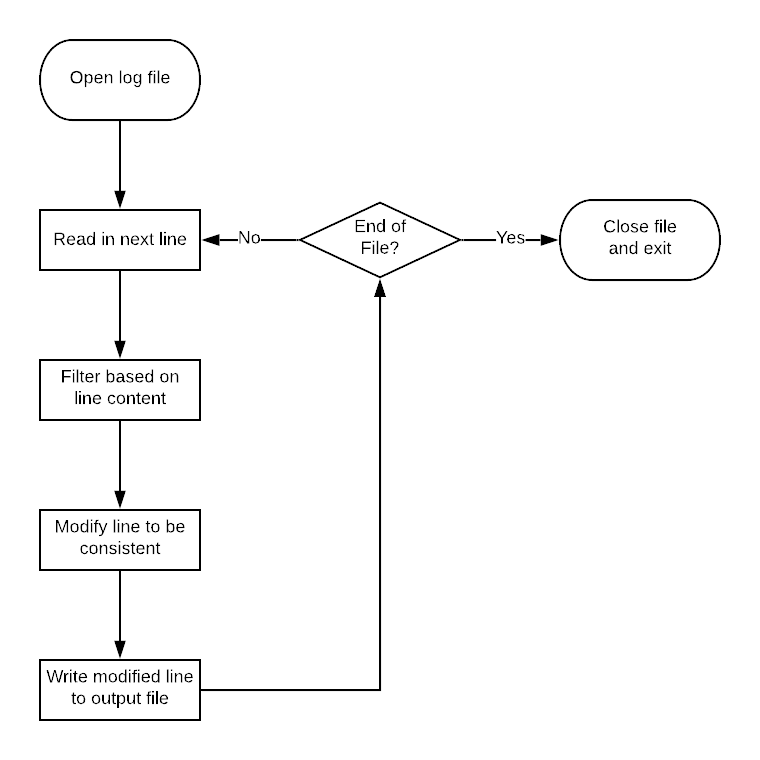
\includegraphics[width=10cm,height=20cm,keepaspectratio]{Figures/Chapter5-SimpleLogFlowchart.png}
        \caption{Flowchart of creating the simple log}
        \label{fig:chapter5SimpleFlowchart}
    \end{centering}
\end{figure}

\pagebreak
\subsection{Filtering Lines}\label{filteringLines}
To minimise the lines added to the simple log file, the initial input file needs to be filtered.
This allows for only specific lines to be added to the log file by adding only the lines which meet specific criteria. 

To determine the minimal information required to understand the tests, the output log files of the tests were analysed.
While analysing the output log files, the following list of important events was created.
\begin{itemize}
    \item \textbf{Setup} Start of a process, LBARD/Fakeradio
    \item \textbf{Setup} Test details
    \item \textbf{Setup} Layout information (WiFi and Fakeradio)
    \item \textbf{Setup} SID information
    \item \textbf{Servald} Sending and receiving packets
    \item \textbf{Servald} Adding manifest
    \item \textbf{LBARD} Neighbour has a bundle
    \item \textbf{LBARD} Send and receive bundles
    \item \textbf{Fakeradio} Any transfer between two nodes
\end{itemize}

This list covers all major aspects of a topology test; transfer of bundles, setup and layout information, sending and receiving general packets (including the tree-sync packets), and some internal logic and processing when packets are sent and received.
With only these important events, it should be possible to locate and isolate issues related to transferring bundles and packets. 
From there, these filtered events should allow a tester to more easily utilise the vastly more expansive and detailed original log file produced by the test framework. 

Once the desired events had been determined, these then needed to be filtered within the program.
To achieve this, each line in the file is analysed to determine if it is important by examining what substrings the line contains.
A line is accepted if it matches specified criteria; for instance, a line within the Fakeradio process that contains the substring "\texttt{neighbour has a bundle}" would be considered important. 
These lines are then sent to the relevant function to be formatted appropriately.

\subsection{Output format}

\subsubsection{Formatting lines}
The log files produced by the test framework follow a consistent structure.
The structure always follows the structure of:
\begin{itemize}
    \item the test details, 
    \item the output of the test framework, 
    \item output of Fakeradio, 
    \item output of \emph{each} LBARD process, and finally,
    \item the output of \emph{each} Servald process.
\end{itemize} 

As this structure is consistent throughout tests in the framework, this allows the tools to only track which process is being processed, and then filter lines based on this.
However, the test framework log files have one major issue: the format of lines is not consistent between processes.
For instance, the typical Servald line may appear as
\begin{center}
    \begin{lstlisting}[basicstyle=\small, breaklines]
DEBUG:[511710] 18:15:34.372 overlay_mdp.c:859:_overlay_send_frame() {mdprequests} Send frame 68 bytes    
    \end{lstlisting}
\end{center}
while a similar line in LBARD follows a format of:
\begin{center}
    \begin{lstlisting}[basicstyle=\small, breaklines]
T+25138ms : Sending length of bundle 6A1A3379501553D1* (bundle #0, version 1596098704035, cached_version 1596098704035)
    \end{lstlisting}
\end{center}

As shown above, the format between these two lines is clearly different and as such need to be formatted differently.
To achieve this, when a line is filtered as outlined in the previous section, the program returns an integer value representing the type of line that is to be formatted.
With this information, the appropriate formatting function can be called for the line type, so that it can be formatted correctly.

For \texttt{servald} lines this is trivial, the C standard function \texttt{sscanf} is used to extract the important information from the line and this information is then written to the simple log output file \texttt{sprintf}.

However, in the case of LBARD and Fakeradio lines, multiple issues arise due to the formatting of the log files.
The first of these issues is that several lines in LBARD are not timestamped with the time that they occurred, rather they are timestamped with the number of milliseconds since the program started as shown above.
This is an issue since this means that the log files can not be easily sorted by timestamp, and also will not be formatted with a consistent format with the other lines.
To fix this, the initial time that an LBARD instance is started as logged by the file will be used as the T=0 point.
After this has occurred, when an event with a 'T+' timestamp is encountered, the number of milliseconds is added to the original timestamp to produce an accurate timestamp for this event.

The other issue with this method is that Fakeradio log lines often are spread over multiple lines.
This means that simply scanning and processing a single line will not produce all the necessary information.
However, this can be mitigated by iterating over several lines until the end of this log line is reached.
As the program iterates through these lines it simply scans for the important information and forms a single log message from this.

With these outliers accounted for, the tool is now able to filter each log line in the initial log file and format these appropriately.


\subsubsection{Output log file}
With this, the log file produced now has a consistent format.
The simple log files format begins with the setup section.
The setup section lists all the essential information for drawing a diagram of the network topology. 
It lists the test details, SIDs of each of the nodes, and all the WiFi connections and Fakeradio rules. 
An example of the setup section can be seen in \figurename{ \ref{fig:chapter5SimpleLogSetup}}.

\begin{figure}
    \begin{centering}
\begin{lstlisting}[frame=single]
#000 ====== BEGIN SETUP ======
#001 Name:     Wifi_RFD900_Chain_Short (topologies)
#002 Result:   PASS
#003 Started:  2020-08-24 13:22:55.044
#004 Finished: 2020-08-24 13:23:32.497
#005 SIDA : F170309E3033B957*
#006 SIDB : 86C9DD08EA6A4C65*
#007 SIDC : FA71E8E919914B52*
#008 SIDD : 41A35E8851578F82*
#009 SIDE : 954B6D94024986A0*
#010 SIDF : B38FB12CB39D006C*
#011 B connected to wifi interface 1
#012 C connected to wifi interface 1
#013 D connected to wifi interface 2
#014 E connected to wifi interface 2
#015 RULE: 'allow between 0,1'
#016 RULE: 'allow between 2,3'
#017 RULE: 'allow between 4,5'
#018 RULE: 'deny all'
#100 ======= END SETUP =======    
\end{lstlisting}
    \caption{Format of simple log setup}
    \label{fig:chapter5SimpleLogSetup}
    \end{centering}
\end{figure}

After the setup section each line in the log file is ordered by chronological order. 
The lines follow a simple and consistent structure.
\begin{center}
    \begin{lstlisting}[basicstyle=\small, breaklines]
[Timestamp] [Process]:[Instance Letter] [Description]
    \end{lstlisting}
\end{center}

This structure can be seen in \figurename{ \ref{fig:chapter5SimpleLogFormat}}.
\begin{figure}
    \begin{centering}
\begin{lstlisting}[basicstyle=\small, breaklines, frame=single]
13:23:18.358 LBARD:A Resending bundle 3580786E* from the start.
13:23:18.358 LBARD:A Sending length of bundle 3580786E* 
13:23:18.370 FAKERADIO A -> B [Bundle end piece ] [218 bytes]
13:23:18.370 FAKERADIO A -> B [Time stamp] [218 bytes]
13:23:18.370 LBARD:A I just sent manifest piece [128,258) for 86c9dd08ea6a*.
13:23:18.388 LBARD:B : Calling message handler for type 'S' @ offset 0x15
13:23:18.388 LBARD:B : Calling message handler for type 'T' @ offset 0x8
13:23:18.388 LBARD:B : Calling message handler for type 'p' @ offset 0x21
13:23:18.388 LBARD:B Decoding message #4 from f170309e3033*, length = 186:
13:23:18.388 LBARD:B We have the entire bundle 3580786E*    
\end{lstlisting}
        \caption{Format of simple log events}
        \label{fig:chapter5SimpleLogFormat}
    \end{centering}
\end{figure}


\section{Drawing Packet Transfer through the network}
To improve the output of the test framework, a network diagram displaying packet transfer is highly useful, allowing testers to better understand the topology they are testing. 
To produce a useful and informative network diagram, four steps need to be undertaken: determine the major events to be displayed on the diagram, create an ASCII representation of events during a test, generate a network diagram, and finally, create a PDF of the network topology with the traffic displayed.

\subsection{Getting Major and Minor events}
Before the network diagrams can be generated, the content that will be displayed must first be determined.
To do this, two categories of log events are defined: 
\begin{list}{}{}
    \item Major: When a node sends a message/packet to another
    \item Minor: Some processing on a single node that would not give the full picture of the test if omitted
\end{list}

Major events will be displayed in a diagram showing the network layout, showing the transfer between the two nodes and the message details. 
Minor events will be displayed in a list of minor events that occurred before the major event.
There can be multiple minor details per major event, however there is only one major event for each minor event.

There are two options for processing and sorting major and minor events.
The first is to process the simple log after it has been made, and check if a line should be considered major or minor. 
The other solution is to classify lines as they are processed in the creation of the simple log.
The second option is considerably faster, as in the first option we must re-process a new file and then classify lines within it to be major or minor, however the second option has a major issue in that when lines are classified during the creation of the simple log they are not yet sorted as the original log file is not sorted.
This means that if an array of major and minor events is created then these events will \emph{not} be in chronological order.
Unsorted events is an issue for the creation of diagrams as the created diagrams will then not be ordered.
This means that for the second option to be considered, a method of sorting and \emph{then} assigning minor events to a major event must be developed.
This is the approach that this thesis took.

Determining major events is simple; major events are a transfer between two nodes.
To save these major events, a struct defining major events is created.
This struct contains all the necessary features of a major event. These details are:
\begin{itemize}
    \item Sending Node
    \item All Destination Nodes
    \item Transfer details (type of message, size, etc.)
    \item The time it occurs at
    \item The transfer type (LBARD or WiFi)
    \item An array of minor events associated with this major event
\end{itemize}
Major events occur at two different points in the log file: when \texttt{fakeradio} sends a packet to a different node, and when \texttt{servald} sends a packet.
\texttt{Fakeradio} events are already filtered down to a one line log event for the simple log, so the program simply breaks this line down to get the details of the event, and then appends this to the major events array.
\texttt{Servald} events however are more complicated as the packet transfer takes place over several messages.
To convert this into one event, the program saves the details of the packet as each line is processed until the log line stating that the message is sent, at which point all the saved details are added to an event and appended to the major event array.

To add the minor events, when a line for the simple log is being formatted for the simple log, the program simply checks if it meets a handful of criteria.
Since the log lines are just a single line, saving these minor events is as simple as appending these lines to the minor event array.


Once the simple log file has been produced, and all major and minor events have been extracted, each minor event needs to be associated with a major event.
When major and minor events are added to their respective arrays, they are done so in the order that the relevant lines appear in the input log file, meaning that these arrays are not chronologically sorted.
To associate a minor event with a major event, the minor event must occur before a major event, but \emph{after} the proceeding major event.
To achieve this, both of the arrays are sorted using the C standard function \texttt{qsort} with a comparator implemented that orders these by timestamp.

With the arrays sorted each minor array can be assigned to a major event.
This is done by assigning each minor event to a specific major event until this minor event occurs after the major event, at which point the next major event is chosen.
This iterates until every major event has had minor events assigned.
Any remaining minor events are assigned to a blank major event.

At this point, an array of all events throughout the test has been created with every minor event assigned to the appropriate major event.


\subsection{ASCII Network Traffic}
Creating an ASCII representation of the network traffic is trivial once minor and major events have been created.
To achieve this, the program simply iterates through every major event.
For each major event, the program then iterates through each minor event associated with this major event.
With this, the program is able to quickly print an ASCII representation of the network traffic through the network during a test.
This can be seen in \figurename{ \ref{fig:chapter5ASCIIRep}}.

\begin{figure}
    \begin{centering}
\begin{lstlisting}[numbers=left, basicstyle=\small, frame=single, breaklines, ]
38: [ 16:12:58.834] Tree sync message
    D -> BROADCAST
- 16:12:58.562 : LBARD:C We have new bundle 57E1F321*

39: [ 16:12:58.835 ] [LBARD instance identifier] [57 bytes]
    D -> C

40: [ 16:12:58.863] Tree sync message
    B -> BROADCAST
- 16:12:58.846 : LBARD:C Neighbour Node D (E31FC729) is missing bundle 57E1F321*
\end{lstlisting}
    \caption{ASCII Representation of test network}
    \label{fig:chapter5ASCIIRep}
    \end{centering}
\end{figure}
This output can then be piped to a file for debugging if testers do not have the requirements installed for generating the diagrams as outlined in the next sections.


\subsection{Generating a network diagram}
\todo{cut down}
To render these diagrams, the network topology needs to be extracted from the test definition, then a diagram drawn of this topology.
From this layout, the image will then need to be created and rendered.
There are two main solutions for creating the image: do it using a graphics library, or creating a DOT file and rendering it with Graphviz.
Using a graphics library would provide a high level of control over the creation of the image as graphical elements would need to be defined explicitly and as such are unlikely to have unforeseen side effects as could be expected with using a higher-level solution such as Graphviz.
However, this would be considerably more complicated and harder to maintain than simply writing DOT files, then using the high-level tools provided by Graphviz to render this DOT file.
DOT files are text files that follow a specified syntax, and are used by Graphviz to render and create graphs.
These files are simple, and both human and machine-readable. 
It was decided that despite the far higher level of control possible by using a low-level graphics library, the accessibility, simplicity and maintainability of creating and rendering DOT files far outweighs this advantage.

To create this diagram, the topology information needs to be extracted from the test log.
For WiFi topologies, the test framework reports whenever a node is connected to a WiFi interface.
To create a diagram every time a node is connected to an interface, the interfaces that a specific node is connected to is saved in an array for each node.
To determine \texttt{fakeradio} topologies, when the \texttt{fakeradio} rules are reported in the log file, the links between nodes are extracted and this information added to a struct.
With this, the links between nodes have been determined, and a network diagram can be generated.

Once the simple log has finished being generated and the links between nodes gathered, the program then moves onto writing the layout DOT file.
The DOT file follows a simple format; initialisation of graph variables, and then the definition of the Layout sub-graph.
The graph is defined as a \emph{directed} graph.
This graph is defined as directed (but with arrow direction hidden) for the use in the network diagrams showing network traffic that will be discussed in the next section.

Producing the DOT file consists of four steps:
\begin{enumerate}
    \item Open the file and initialise variabls
    \item Write the Fakeradio links
    \item Write the WiFi nodes
    \item Write the end of the DOT file, then close it
\end{enumerate}

In the first step, the program opens a new file with the name \texttt{diagramLayout.dot}, and writes the initialisation variables.
The initialisation variables are the padding around the image the pen width to be used for drawing the diagram.

In the next step, the program simply iterates through each \texttt{fakeradio} link and defines a dashed link between these two nodes and colours it red.
This is used to highlight Fakeradio links between nodes and help distinguish the different link types between nodes in a network.


Then, the program iterates through the WiFi link array. 
To do this, the program iterates through each of the interface arrays, and for each, defines a dashed link for all \emph{unique} combinations of the nodes in this interface which are then coloured blue.

Finally, the program adds the closing curly braces to the file, and closes it.
The program then renders the DOT file with the command:

\texttt{neato -Tpng [fileName] -o [outputFileName]}

With this, the tool is able to create network topology diagrams using just the log information.

\begin{figure}
    \begin{centering}
        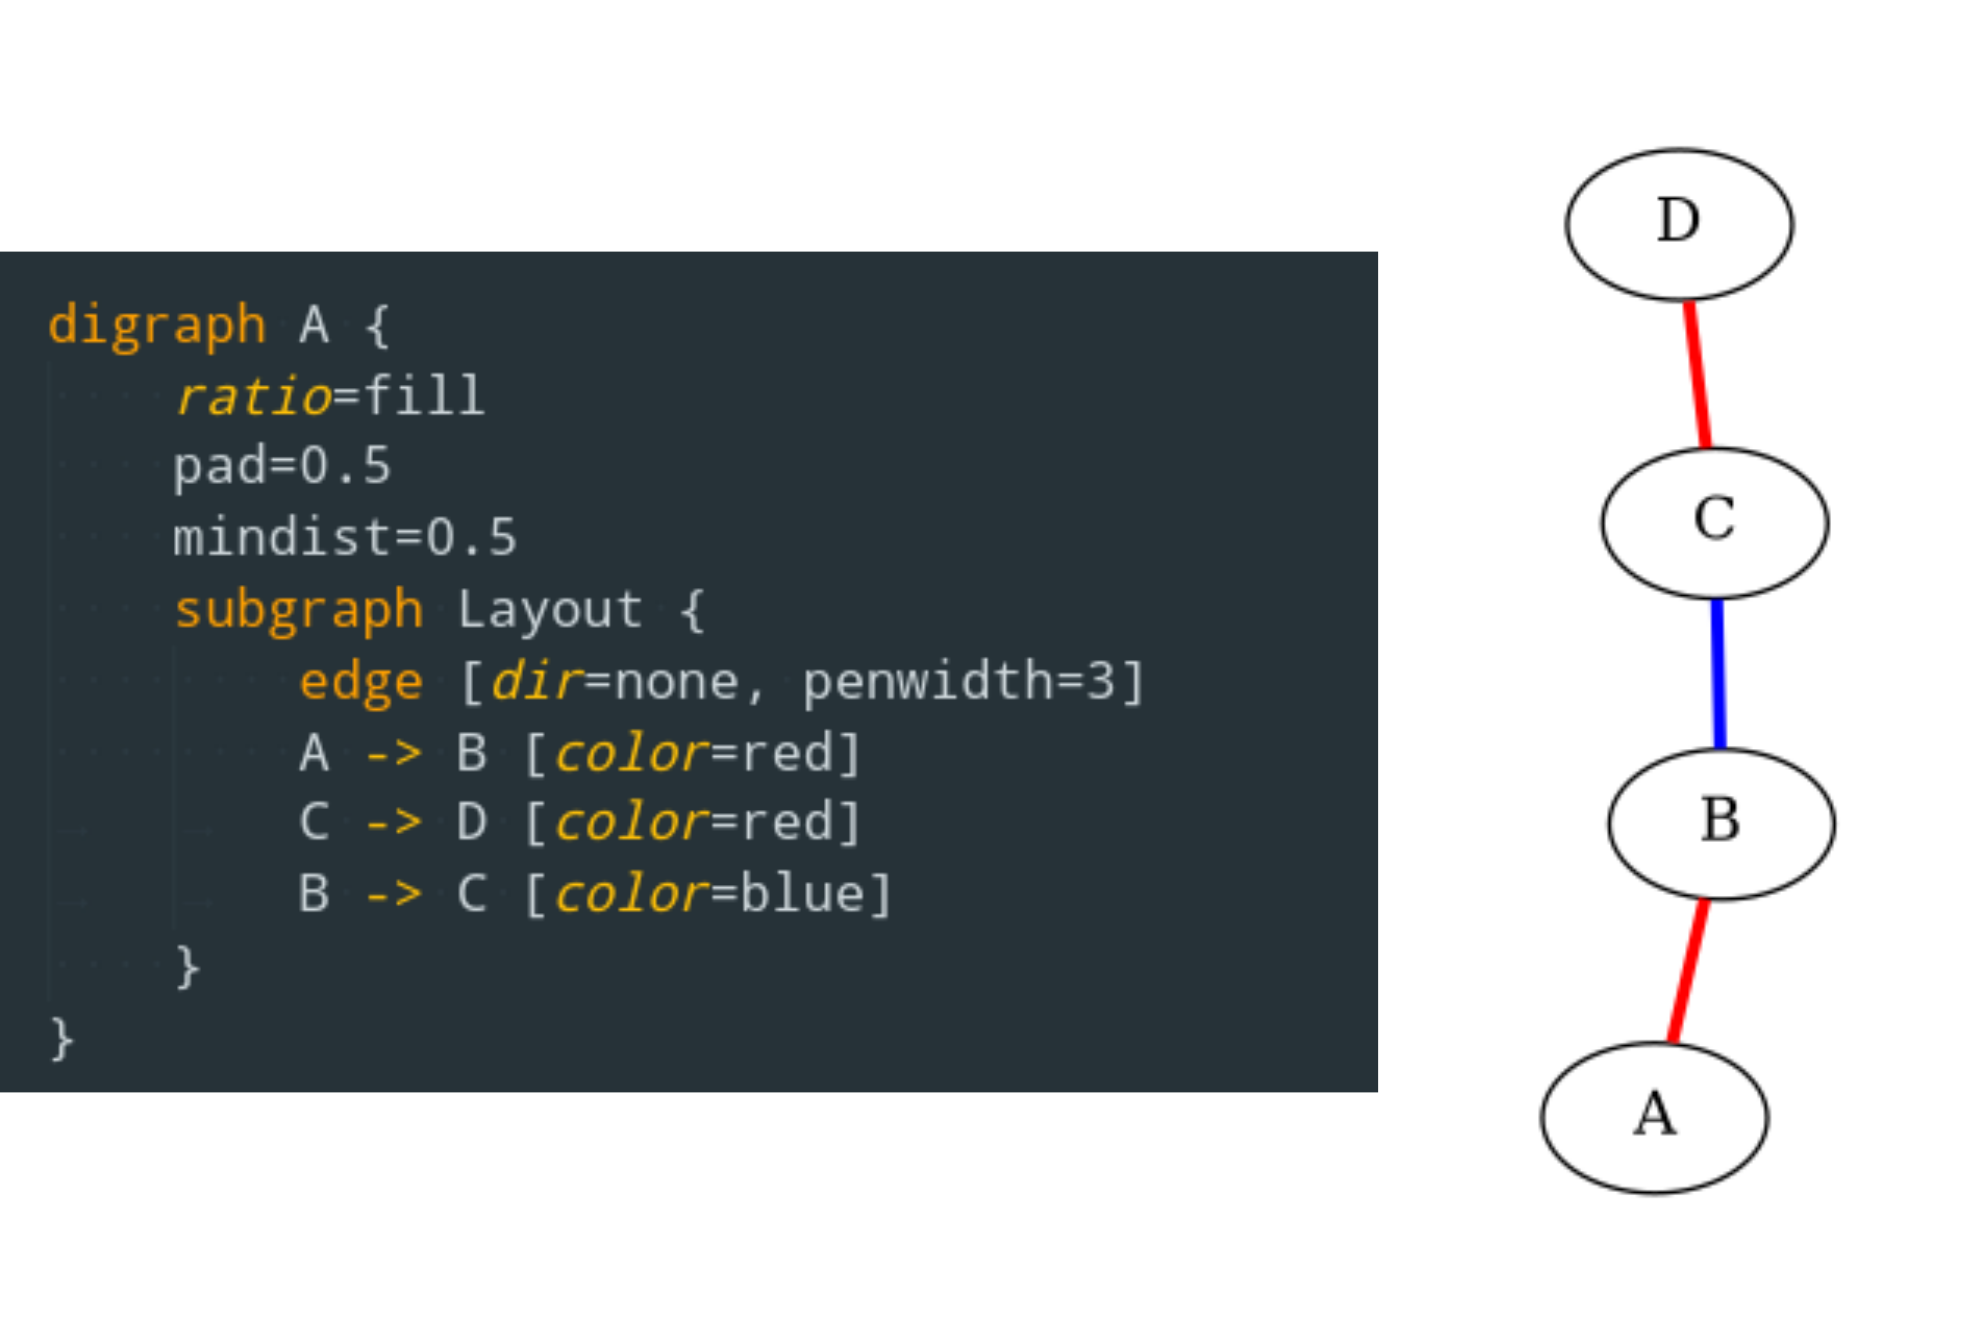
\includegraphics[width=15cm,height=10cm,keepaspectratio]{Figures/Chapter5-DotAndRender.png}
        \caption{Side-by-side of DOT file and output graph\\\emph{Rendered using neato}}
        \label{fig:chapter5DotAndRender}
    \end{centering}
\end{figure}
\todo{Move this to a lstlisting next to an image}

\subsection{Creating a LaTeX PDF}
To generate PDFs of the network traffic throughout the test, two steps must be made: create diagrams for each major event showing the network traffic during this major event, then add these diagrams and all minor events to a LaTeX template which is then rendered to a PDF.

\subsubsection{Transfer Diagrams}
The first step in creating a LaTeX PDF is to generate all the images of the network topology.
This is an extension of the development done in the previous section, however this is now creating multiple images — one per major event — and adding a directed link and label between a sending and receiving node.

To achieve this, the program iterates through every single major event and creates a new DOT file for each event.
In each file, the DOT file is created as previously outlined, however a new subgraph is added named \emph{Transfer}
The transfer sub-graph contains a single solid line definition of a \emph{directed} connection between the sending and receiving node.
To display the transfer on this directed link between the nodes, a label is added that displays the transfer message.

With this, the DOT file can be compiled as previously described to generate a diagram for each major event.
When these are compiled in the LaTeX PDF this will have the effect of appearing to animate the network topology.


\subsubsection{Creating the LaTeX PDF}
Once the diagrams have been created, a LaTeX PDF can then be created.
This PDF contains several pieces of information:
\begin{itemize}
    \item The test details
    \item A diagram for each major event
    \item All minor events associated with that major event
    \item The time the major event occurs
\end{itemize}
The produced LaTeX file follows a simple structure.
At the top of every page, the details of the test (name, result, and start/finish time) are listed.
Underneath this, the time that the major event occurred is listed. 
The vast majority of the page is taken up by the diagram of the network layout, showing the network traffic when the major event occurs.
Finally, the bottom half of the page is a list of minor events associated with the major event.

To produce this, the program follows a simple process.
For the first major event, the program creates a new LaTeX file and writes the import and setup lines necessary for the compilation of the LaTeX document.
Then, the program simply writes the test details to the file with the \texttt{\\large} tag.
The program then adds the image for that major event to the file. 
After this, the program simply iterates through every minor event associated with the major event, and adds these lines to the LaTeX file.
Finally, a page break is added so that the next major event is put on a new page.
This is done for every major event.

Once the LaTeX file has been produced, the program renders the file using the command
\texttt{pdflatex --output-directory=[output file] [file]}
This then creates a PDF where each page displays the network traffic during a major event, and lists all the minor events associated with this major event.

\section{Summary}

In this chapter we have continued answering the fourth research question: "\fourthRQ" as started in Chapter \ref{Chapter4}.
These additional diagnostic tools were in the form of a C program that could be used to generate simpler, formatted, and chronologically ordered log files from the log files produced by the test framework.
This tool allows for the log file produced by the test framework to be processed and a simpler and clearer log file produced from this.
This tool also provided two methods of displaying the network topology throughout these tests in the form of ASCII and PDFs.
The ASCII output provides testers who lack the requirements required for the PDF generation (GraphViz and LaTeX) to perform analysis of these networks without external requirements.
The PDF output allows testers to visually analyse the network traffic during a test and provides the basis for determining where faults are occurring.

In this chapter the outputs of the test framework were improved based on the improvements outlined in Chapter \ref{Chapter3}.
In the next chapter, the tools developed in this chapter will be improved to model real-world Serval networks, and the basis for analysing the differences between real-world and emulated tests described.
